\section{Lernziele}
Zu Beginn jedes Kapitel (bis auf das erste) werden im Lernskript jeweils die Lernziele, sowie die Aufgaben welche diese abdecken, aufgelistet.
Dies zeigt den Lernenden auf, was wichtig ist und was von ihnen erwartet wird.
So können Sie ihre Lernzeit gezielter investieren.
Damit die Lernenden ihren eigenen Fortschritt prüfen können, wird zu jedem Lernziel mindestens eine Aufgabe gestellt.

Lernziele können gemäss der revidierten Taxonomie von Bloom klassifizert werden~\cite{Bloom1956},~\cite{Anderson2001}.
Die verschiedenen Klassen sind in Abbildung~\ref{fig:taxonomie} aufgelistet.
\begin{figure}[ht]
	\centering
	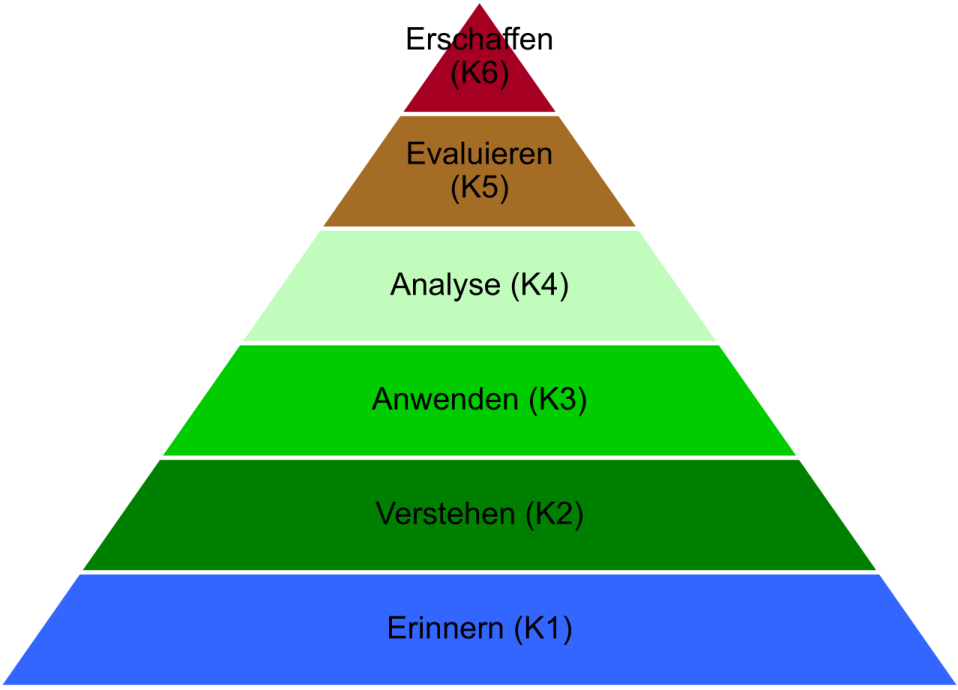
\includegraphics[width=0.5\textwidth]{images/taxonomie}
	\caption{Blooms revidierte Taxonomie von Lernzielen~\cite{Anderson2001}.}
	\label{fig:taxonomie}
\end{figure}
Alle Lernziele aus dem Lernskript sind in Tabelle~\ref{tab:lernziele} nochmals aufgelistet und gemäss dieser Taxonomie klassifiziert.
\begin{table}[ht]
	\centering
	\begin{tabular}{|l|l|}
		\hline
		Klassifizierung & Lernziele \\ \hline
		Wissen &  \\
		Verstehen & \ref{item:hmmc}, \ref{item:eigenfaces}, \ref{item:compression_theory}, \ref{item:recognition}  \\
		Anwenden & \ref{item:vectormatrix_theory}, \ref{item:vectormatrix_code}, \ref{item:meandiff_simple}, \ref{item:meanface}, \ref{item:distance}, \ref{item:projection}, \ref{item:compute_coefficients}, \ref{item:compression_code}  \\
		Analyse &  \\
		Evaluieren &  \\
		Erschaffen &  \\
		\hline
	\end{tabular} %\ref{item:scaling}, \ref{item:projection_3d}, 
	\caption{Klassifizierung der Lernziele aus dem Skript.}
	\label{tab:lernziele} 
\end{table}